\documentclass[10pt]{article}
\usepackage{tikz}
\usetikzlibrary{positioning,arrows}
\usetikzlibrary{shapes.geometric}
\usepackage{geometry}
%\tikzstyle{v}=[draw, inner sep=6pt, minimum size=6pt, node distance=2.5cm]
\tikzstyle{w}=[draw, circle, inner sep=8pt, minimum size=6pt, node distance=2.5cm, fill = lightgray]
%\tikzstyle{ws}=[draw, circle, inner sep=6pt, minimum size=6pt, node distance=2.5cm, fill = lightgray]
\tikzstyle{u}=[draw, circle, inner sep=8pt, minimum size=6pt, node distance=2.5cm]

\begin{document}
\begin{figure}[h]
	\centering
	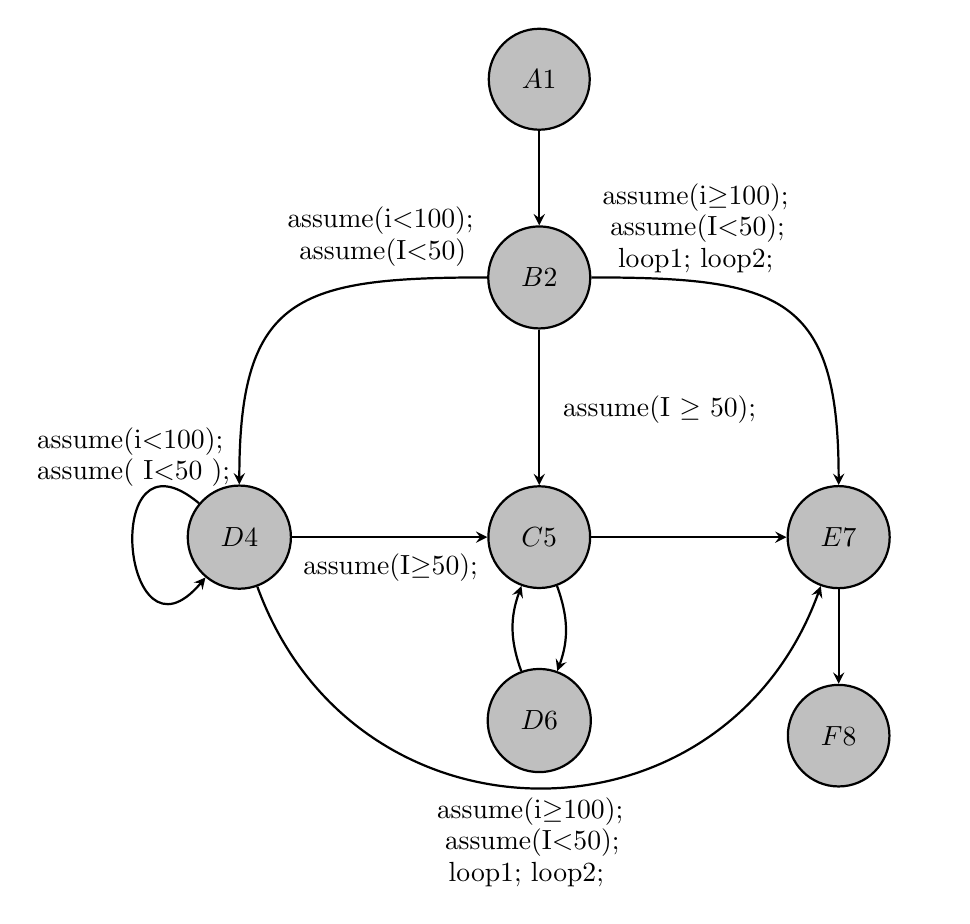
\begin{tikzpicture}[scale=1.0,transform shape, -triangle 45, thick]
	%\node[w] (A1) at ( -6, 5) {$A1$}; 
	%\node[w] (B2) [right of = A1] {$B2$};
	%\node[w] (D4) [right = 3cm of B2] {$D4$};
	\node[w] (Hi) at (0,10) {$A1$};
	\node[w] (Yo) [below = 1.2cm of Hi] {$B2$};
	\node[w] (Ya) [below = 4.5cm of Hi] {$C5$};
	\node[w] (Da) [left = 2.48cm of Ya] {$D4$};
	\node[w] (Ga) [right = 2.48cm of Ya] {$E7$};
	\node[w] (Pa) [below = 1.2cm of Ga] {$F8$};
	\node[w] (La) [below = 1cm of Ya] {$D6$};
	\node[text width=4cm] at (0.7,0.7) {assume(i$\geq$100);};
	\node[text width=4cm] at (0.8,0.3) {assume(I$<$50);};
	\node[text width=4cm] at (0.85,-0.1) {loop1; loop2;};
	\node[text width=4cm] at (-1,3.8) {assume(I$\geq$50);};
	\node[text width=4cm] at (-4.38,5.4) {assume(i$<$100);};
	\node[text width=4cm] at (-4.38,5) {assume( I$<$50 );};
	\node[text width=4cm] at (2.3,5.8) {assume(I $\geq$ 50);};
	\node[text width=4cm] at (-1.05,7.8) {assume(I$<$50)};
	\node[text width=4cm] at (-1.2,8.2) {assume(i$<$100);};
	\node[text width=4cm] at (2.8,8.5) {assume(i$\geq$100);};
	\node[text width=4cm] at (2.9,8.1) {assume(I$<$50);};
	\node[text width=4cm] at (3,7.7) {loop1; loop2;};
	
	\draw (Hi) edge[->,>=stealth] (Yo);
	\draw (Yo) edge[->,>=stealth] (Ya);
	\draw (Da) edge[->,>=stealth] (Ya);
	\draw (Ya) edge[->,>=stealth] (Ga);
	\draw (Yo) edge[->,>=stealth,out=180,in=90,looseness=1.5] (Da);
	\draw (Yo) edge[->,>=stealth,out=0,in=90,looseness=1.5] (Ga);
	\draw (Ga) edge[->,>=stealth] (Pa);
	\draw (La) edge[->,>=stealth,out=110,in=250] (Ya);
	\draw (Ya) edge[->,>=stealth,out=290,in=70] (La);
	\draw (Da) edge[->,>=stealth,out=140,in=230,looseness=4.5] (Da);
	\draw (Da) edge[->,>=stealth,out=290,in=250,looseness=1.3] (Ga);
	
	\end{tikzpicture}
  \label{fig:sat-reduction-edges}
\end{figure}
\end{document}
